% GNUPLOT: LaTeX picture with Postscript
\begingroup
  \makeatletter
  \providecommand\color[2][]{%
    \GenericError{(gnuplot) \space\space\space\@spaces}{%
      Package color not loaded in conjunction with
      terminal option `colourtext'%
    }{See the gnuplot documentation for explanation.%
    }{Either use 'blacktext' in gnuplot or load the package
      color.sty in LaTeX.}%
    \renewcommand\color[2][]{}%
  }%
  \providecommand\includegraphics[2][]{%
    \GenericError{(gnuplot) \space\space\space\@spaces}{%
      Package graphicx or graphics not loaded%
    }{See the gnuplot documentation for explanation.%
    }{The gnuplot epslatex terminal needs graphicx.sty or graphics.sty.}%
    \renewcommand\includegraphics[2][]{}%
  }%
  \providecommand\rotatebox[2]{#2}%
  \@ifundefined{ifGPcolor}{%
    \newif\ifGPcolor
    \GPcolortrue
  }{}%
  \@ifundefined{ifGPblacktext}{%
    \newif\ifGPblacktext
    \GPblacktextfalse
  }{}%
  % define a \g@addto@macro without @ in the name:
  \let\gplgaddtomacro\g@addto@macro
  % define empty templates for all commands taking text:
  \gdef\gplbacktext{}%
  \gdef\gplfronttext{}%
  \makeatother
  \ifGPblacktext
    % no textcolor at all
    \def\colorrgb#1{}%
    \def\colorgray#1{}%
  \else
    % gray or color?
    \ifGPcolor
      \def\colorrgb#1{\color[rgb]{#1}}%
      \def\colorgray#1{\color[gray]{#1}}%
      \expandafter\def\csname LTw\endcsname{\color{white}}%
      \expandafter\def\csname LTb\endcsname{\color{black}}%
      \expandafter\def\csname LTa\endcsname{\color{black}}%
      \expandafter\def\csname LT0\endcsname{\color[rgb]{1,0,0}}%
      \expandafter\def\csname LT1\endcsname{\color[rgb]{0,1,0}}%
      \expandafter\def\csname LT2\endcsname{\color[rgb]{0,0,1}}%
      \expandafter\def\csname LT3\endcsname{\color[rgb]{1,0,1}}%
      \expandafter\def\csname LT4\endcsname{\color[rgb]{0,1,1}}%
      \expandafter\def\csname LT5\endcsname{\color[rgb]{1,1,0}}%
      \expandafter\def\csname LT6\endcsname{\color[rgb]{0,0,0}}%
      \expandafter\def\csname LT7\endcsname{\color[rgb]{1,0.3,0}}%
      \expandafter\def\csname LT8\endcsname{\color[rgb]{0.5,0.5,0.5}}%
    \else
      % gray
      \def\colorrgb#1{\color{black}}%
      \def\colorgray#1{\color[gray]{#1}}%
      \expandafter\def\csname LTw\endcsname{\color{white}}%
      \expandafter\def\csname LTb\endcsname{\color{black}}%
      \expandafter\def\csname LTa\endcsname{\color{black}}%
      \expandafter\def\csname LT0\endcsname{\color{black}}%
      \expandafter\def\csname LT1\endcsname{\color{black}}%
      \expandafter\def\csname LT2\endcsname{\color{black}}%
      \expandafter\def\csname LT3\endcsname{\color{black}}%
      \expandafter\def\csname LT4\endcsname{\color{black}}%
      \expandafter\def\csname LT5\endcsname{\color{black}}%
      \expandafter\def\csname LT6\endcsname{\color{black}}%
      \expandafter\def\csname LT7\endcsname{\color{black}}%
      \expandafter\def\csname LT8\endcsname{\color{black}}%
    \fi
  \fi
  \setlength{\unitlength}{0.0500bp}%
  \begin{picture}(5102.00,5668.00)%
    \gplgaddtomacro\gplbacktext{%
      \colorrgb{0.31,0.31,0.31}%
      \put(217,3384){\makebox(0,0)[r]{\strut{}\scriptsize 19}}%
      \colorrgb{0.31,0.31,0.31}%
      \put(217,3765){\makebox(0,0)[r]{\strut{}\scriptsize 20}}%
      \colorrgb{0.31,0.31,0.31}%
      \put(217,4145){\makebox(0,0)[r]{\strut{}\scriptsize 21}}%
      \colorrgb{0.31,0.31,0.31}%
      \put(217,4526){\makebox(0,0)[r]{\strut{}\scriptsize 22}}%
      \colorrgb{0.31,0.31,0.31}%
      \put(217,4906){\makebox(0,0)[r]{\strut{}\scriptsize 23}}%
      \colorrgb{0.31,0.31,0.31}%
      \put(217,5287){\makebox(0,0)[r]{\strut{}\scriptsize 24}}%
      \colorrgb{0.31,0.31,0.31}%
      \put(217,5667){\makebox(0,0)[r]{\strut{}\scriptsize 25}}%
      \colorrgb{0.31,0.31,0.31}%
      \put(396,3117){\makebox(0,0){\strut{}}}%
      \colorrgb{0.31,0.31,0.31}%
      \put(762,3117){\makebox(0,0){\strut{}}}%
      \colorrgb{0.31,0.31,0.31}%
      \put(1128,3117){\makebox(0,0){\strut{}}}%
      \colorrgb{0.31,0.31,0.31}%
      \put(1494,3117){\makebox(0,0){\strut{}}}%
      \colorrgb{0.31,0.31,0.31}%
      \put(1859,3117){\makebox(0,0){\strut{}}}%
      \colorrgb{0.31,0.31,0.31}%
      \put(2225,3117){\makebox(0,0){\strut{}}}%
      \colorrgb{0.31,0.31,0.31}%
      \put(2591,3117){\makebox(0,0){\strut{}}}%
      \colorrgb{0.31,0.31,0.31}%
      \put(2957,3117){\makebox(0,0){\strut{}}}%
      \colorrgb{0.31,0.31,0.31}%
      \put(3323,3117){\makebox(0,0){\strut{}}}%
      \colorrgb{0.31,0.31,0.31}%
      \put(3689,3117){\makebox(0,0){\strut{}}}%
      \colorrgb{0.31,0.31,0.31}%
      \put(4054,3117){\makebox(0,0){\strut{}}}%
      \colorrgb{0.31,0.31,0.31}%
      \put(4420,3117){\makebox(0,0){\strut{}}}%
      \colorrgb{0.31,0.31,0.31}%
      \put(4786,3117){\makebox(0,0){\strut{}}}%
      \csname LTb\endcsname%
      \put(-157,4525){\rotatebox{-270}{\makebox(0,0){\strut{}$P(1,2)$ (\%)}}}%
      \put(2682,3051){\makebox(0,0){\strut{}}}%
      \put(2774,5484){\makebox(0,0)[l]{\strut{}\scriptsize$\lambda_{ir}=0.1263$}}%
    }%
    \gplgaddtomacro\gplfronttext{%
    }%
    \gplgaddtomacro\gplbacktext{%
      \colorrgb{0.31,0.31,0.31}%
      \put(217,751){\makebox(0,0)[r]{\strut{}\scriptsize 0}}%
      \colorrgb{0.31,0.31,0.31}%
      \put(217,1145){\makebox(0,0)[r]{\strut{}\scriptsize 2}}%
      \colorrgb{0.31,0.31,0.31}%
      \put(217,1540){\makebox(0,0)[r]{\strut{}\scriptsize 4}}%
      \colorrgb{0.31,0.31,0.31}%
      \put(217,1934){\makebox(0,0)[r]{\strut{}\scriptsize 6}}%
      \colorrgb{0.31,0.31,0.31}%
      \put(217,2328){\makebox(0,0)[r]{\strut{}\scriptsize 8}}%
      \colorrgb{0.31,0.31,0.31}%
      \put(217,2723){\makebox(0,0)[r]{\strut{}\scriptsize 10}}%
      \colorrgb{0.31,0.31,0.31}%
      \put(217,3117){\makebox(0,0)[r]{\strut{}\scriptsize 12}}%
      \colorrgb{0.31,0.31,0.31}%
      \put(396,484){\makebox(0,0){\strut{}\scriptsize 0}}%
      \colorrgb{0.31,0.31,0.31}%
      \put(762,484){\makebox(0,0){\strut{}\scriptsize 0.02}}%
      \colorrgb{0.31,0.31,0.31}%
      \put(1128,484){\makebox(0,0){\strut{}\scriptsize 0.04}}%
      \colorrgb{0.31,0.31,0.31}%
      \put(1494,484){\makebox(0,0){\strut{}\scriptsize 0.06}}%
      \colorrgb{0.31,0.31,0.31}%
      \put(1859,484){\makebox(0,0){\strut{}\scriptsize 0.08}}%
      \colorrgb{0.31,0.31,0.31}%
      \put(2225,484){\makebox(0,0){\strut{}\scriptsize 0.1}}%
      \colorrgb{0.31,0.31,0.31}%
      \put(2591,484){\makebox(0,0){\strut{}\scriptsize 0.12}}%
      \colorrgb{0.31,0.31,0.31}%
      \put(2957,484){\makebox(0,0){\strut{}\scriptsize 0.14}}%
      \colorrgb{0.31,0.31,0.31}%
      \put(3323,484){\makebox(0,0){\strut{}\scriptsize 0.16}}%
      \colorrgb{0.31,0.31,0.31}%
      \put(3689,484){\makebox(0,0){\strut{}\scriptsize 0.18}}%
      \colorrgb{0.31,0.31,0.31}%
      \put(4054,484){\makebox(0,0){\strut{}\scriptsize 0.2}}%
      \colorrgb{0.31,0.31,0.31}%
      \put(4420,484){\makebox(0,0){\strut{}\scriptsize 0.22}}%
      \colorrgb{0.31,0.31,0.31}%
      \put(4786,484){\makebox(0,0){\strut{}\scriptsize 0.24}}%
      \csname LTb\endcsname%
      \put(-157,1934){\rotatebox{-270}{\makebox(0,0){\strut{}$P(1,3)$ (\%)}}}%
      \put(2682,154){\makebox(0,0){\strut{}$\lambda_{ir}$ (eV)}}%
      \put(2774,2928){\makebox(0,0)[l]{\strut{}\scriptsize$\lambda_{ir}=0.1263$}}%
    }%
    \gplgaddtomacro\gplfronttext{%
    }%
    \gplbacktext
    \put(0,0){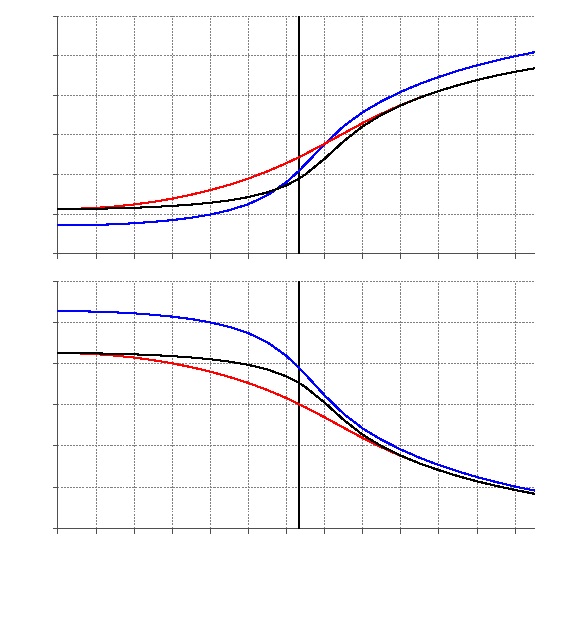
\includegraphics{images/electronicOccupations}}%
    \gplfronttext
  \end{picture}%
\endgroup
